% ------------------------------------------------------------------------
% ------------------------------------------------------------------------
% ------------------------------------------------------------------------
%                            Recomendaciones
% ------------------------------------------------------------------------
% ------------------------------------------------------------------------
% ------------------------------------------------------------------------

\chapter{ESTRUCTURA ELECTRÓNICA Y FONÓNICA DE LAS CONFIGURACIONES MAS ESTABLES}
% ------------------------------------------------------------------------
\section{ESTRUCTURA ELECTRÓNICA}

El inconveniente en usar \textsc{dft} es la descripción incorrecta de la estructura electrónica provocando el llamado "problema de bandagap", subestimando la correlación entre electrones, que a su vez impone dificultades para predecir interacciones intermoleculares precisas, energías de formación y estados de transición \cite{Tolba2018}. Para aumentar la precisión en los cálculos, es necesario introducir el esquema \textsc{dft+u} (Liechtenstein \cite{Lichtenstein1995StrongOrdering}), que es uno de los enfoques correctivos empleados para corregir el "problema de bandgap". Este parámetro se agrega al funcional de la densidad \textsc{gga+u}, corrigiendo la correlación de los electrones en los átomos tántalo y niobio a través de introducir un termino adicional en el hamiltoniano, agregado como una energía en los orbitales y corrige los orbitales y la separación entre ellos.

En esta sección, las estructuras electrónicas son calculadas mediante \textsc{dft} y \textsc{dft+u}, específicamente las configuraciones $Sr_{2}(Ta,Nb)O_{3}N$ \emph{trans} y \emph{cis} de mínima energía, siendo estas $Immm(71)$ y $Cmcm(63)$, respectivamente. Además, se realiza un análisis de la brecha entre la banda de valencia y la banda de conducción, la contribución orbital y una posible aplicación: fotocatálisis para división de agua.  

\section{Relevantes detalles computacionales: Cálculo auto-consistente}

El cálculo auto-consistente es un método iterativo para resolver el problema de valores propios $\epsilon_{i}$ y funciones propias $\Psi_{i}(\vec{r})$ de las ecuaciones de Khon-Sham (ecuación \ref{Eq. KS}) bajo la teoría funcional de la densidad. El problema es que $V_{\text{ext}}$ y $V_{xc}$ dependen de la densidad $n$, y esta a su vez depende de las funciones propias  $\Psi_{i}(\vec{r})$ desconocidas, lo que implica que debe ser determinada de forma auto-consistente.  Para resolver la ecuación de Schrodinger se debe estimar una densidad electrónica inicial $n^{j}(\vec{r})$ agregando las densidades electrónicas de los átomos aislados teniendo en cuenta los sitios atómicos de la estructura. Usando esta densidad obtenemos un primer potencial $V_{\text{Hartree}}+V_{xc}$ que es agregado al potencial de Khom-Sham (ecuación \ref{Eq. V_ks}), y se resuelve el hamiltoniano de Khom-Sham (ecuación \ref{Eq. KS}) discretizando el espacio en punto $k$ para encontrar los valores propios y las funciones propias \cite{lin_lu_ying_2019}. Con estos orbitales encontrados se construye una nueva densidad electrónica $n^{\text{j+1}}(\vec{r})$ y se repite el proceso de forma iterativa hasta que la densidad inicial $n^{j}(\vec{r})$ y la densidad final $n^{\text{j+1}}(\vec{r})$ sean iguales \cite{Woods2018Theory}, es decir, cuando se encuentra el estado base de la densidad electrónica que minimiza el hamiltoniano Khon-Sham \cite{GiustinoFeliciano2014Mmud}.

%Los resultados de los cálculos presentados fueron obtenidos usando la plataforma \texttt{GridUIS-2}, desarrollada por el Centro de Supercomputación y Cálculo Científico de la Universidad Industrial de Santander (\textsc{sc3uis}). Esta acción es soportada por la Vicerrectoría de Investigación y Extensión de la \textsc{uis} (\textsc{vie-uis}) y diferentes grupos de investigación de la universidad. (\url{http://www.sc3.uis.edu.co})

\subsection{Configuración $Sr_{2}(Ta,Nb)O_{3.5}N_{0.5}$  $Pmmm(47)$}

En este caso, la concentración x=0.5 hay pocos reportes en la literatura, así que se determinó si el parámetro \textsc{u} corrigió los orbitales de manera considerable mediante un análisis de estructura de bandas. Se realizó un calculo de bandas para la fase Ruddlesden-Popper $Sr_{2}BO_{3.5}N_{0.5}(B=Ta/Nb)-Pmmm$, que es la estructura de mínima energía. Los resultados son los siguientes:

\begin{figure}[H]
    \centering
    \includegraphics[width=0.4\textwidth]{Figs/bandas-con-u_ta35.eps}
    \includegraphics[width=0.4\textwidth]{Figs/bandas-con-u_nb35.eps}
    \caption{Estructura de bandas electrónicas de la fase Ruddlesden-Popper ($Sr_{2}(Ta,Nb)O_{3}N$).}
    \label{Fig. bandas_35}
\end{figure}

Específicamente en la gráfica \ref{Fig. bandas_35}(b), se observa que en el punto $\Gamma$ se superponen las bandas de conducción $d$ del niobio con las bandas de valencia $p$ del nitrógeno, lo que indican malos resultados computacionalmente. Para ambas gráficas en \ref{Fig. bandas_35}, el supuesto nivel de Fermi que se obtuvo esta en $-1.8  eV$, lo cual es incorrecto, el nivel de Fermi debe estar idealmente en $0 eV$, lo que confirma que el parámetro \textsc{u} falló en corregir los orbitales atómicos. La energía \textsc{u} no corrige adecuadamente los orbitales atómicos de la fase Ruddlesden-Popper $Sr_{2}AO_{3.5}N_{0.5}(B=Ta/Nb)$ debido a la presencia de poco nitrógeno en los octaedros. Se debe realizar un estudio acerca del valor del parámetro \textsc{u} para esta fase, en caso de que la corrección falle se podría recurrir a otras teorías como 'dynamical mean-field theory' \textsc{dmft} combinada con \textsc{dft}.

\subsection{Configuración $Sr_{2}(Ta,Nb)O_{3}N$ \emph{trans} $Immm(71)$}

Los puntos de alta simetría que guían el camino en la zona de Brillouin de la estructura electrónica se obtuvieron mediante el código \textsc{vaspkit} \cite{Wang2019VASPKITCode}:

$$\Gamma-X-F_{2}/\Sigma_{0}-\Gamma-Y_{0}/U_{0}-X/\Gamma-R-W-S-\Gamma-T-W$$

\begin{figure}[H]
    \centering
    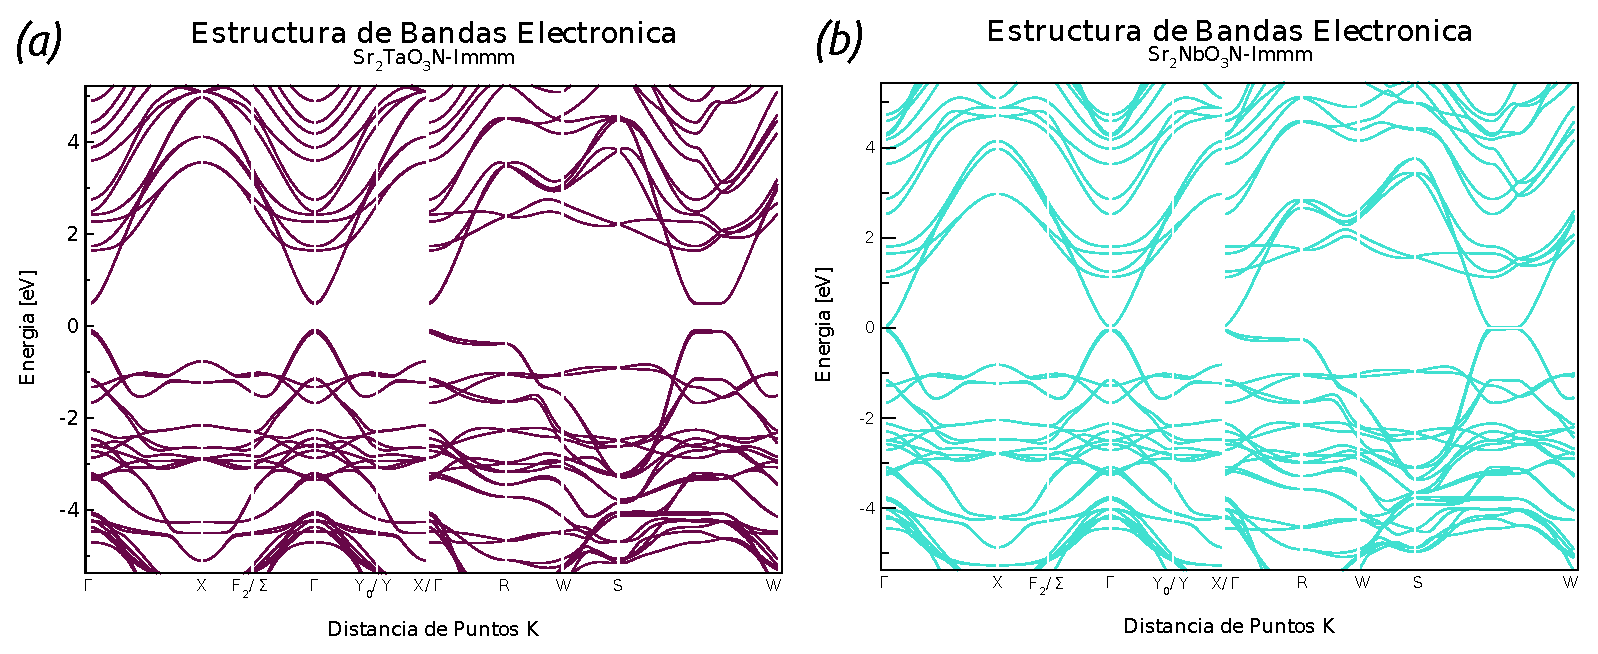
\includegraphics[width=\textwidth]{Figs/bands-trans_sin-U.eps}
    \caption{Estructura de bandas electrónicas de la configuración con ordenamiento aniónico \emph{trans}  (a) $Sr_{2}TaO_{3}N$ y (b) $Sr_{2}NbO_{3}N$, sin tener en cuenta el parámetro \textsc{u}.}
    \label{Fig. bandas_trans-sin-u}
\end{figure}

Al observar principalmente las bandas de conducción y las de valencia en la figura \ref{Fig. bandas_trans-sin-u}(a), la configuración \textsc{rp}$Sr_{2}TaO_{3}N$  muestra un brecha en el punto $\Gamma$ de $0.5728 eV$, lo que indica que el material es aislante. Analizando la figura \ref{Fig. bandas_trans-sin-u}(b) la configuración \textsc{rp}$Sr_{2}NbO_{3}N$ muestra una brecha insignificante de $0.0001 eV$, mostrando un comportamiento conductor, lo cual no van en concordancia con los datos reportados en la literatura \cite{Diot1999CrystalN,Bouri2018}. Por ende, se hace necesario agregar el parámetro \textsc{u} a los cálculos en \textsc{dft}. Dentro del cálculo se tuvo en cuenta el parámetro de corrección \textsc{u} con un valor de $4.0  eV$, los resultados son los siguientes:

\begin{figure}[H]
    \centering
    \includegraphics[width=\textwidth]{Figs/bands-con-u_trans.png}
    \caption{Estructura de bandas electrónica de la configuración con ordenamiento aniónico \emph{trans}  (a) $Sr_{2}TaO_{3}N$ y (b) $Sr_{2}NbO_{3}N$, calculadas mediante \textsc{dft+u} con valor de $U=4.0  eV$}
    \label{Fig. bands-con-u_trans}
\end{figure}

En el caso de las bandas electrónicas de $Sr_{2}TaO_{3}N-Immm$ (figura \ref{Fig. bands-con-u_trans}(a)), el bandgap en el punto $\Gamma$ aumenta a un valor de $1.1202  eV$ comparado con las bandas previas sin el parámetro \textsc{u} donde se obtenía un valor de $0.5728  eV$. Las bandas $d$ del niobio y del tántalo tienen forma parabólica en el punto $\Gamma$, lo que indican buenos resultados. En el caso de las bandas electrónicas de $Sr_{2}NbO_{3}N-Immm$ (figura \ref{Fig. bands-con-u_trans}(b)), el bandgap en el punto $\Gamma$ aumenta a un valor de $0.5194  eV$ comparado con las bandas previas sin el parámetro \textsc{u} donde se obtenía un valor casi nulo. En ambos casos, se evidencia una apertura de la brecha entre la banda de valencia y la banda de conducción, esto debido al parámetro\textsc{u} agregado en los metales de transición.

Para un mayor análisis, se define un camino estándar en la zona de Brillouin para las configuraciones $Sr_{2}(Ta,Nb)O_{3}N$ \emph{trans-}$Immm$ y \emph{cis-}$Cmcm$, con el fin de comparar y especificar los cambios que surgen en las la estructura electrónica. El camino en el espacio $k$ es:

$$(0,0,0)-(0.5,0,0)-(0.5,0.5,0)-(0,0,0)-(0.5,0.5,0.5)-(0,0,0.5)$$

Además, se realiza la proyección atómica de las bandas electrónicas,  es decir, las bandas de los átomos de estroncio, niobio, tántalo, oxigeno y nitrógeno están marcadas con el color indicado en cada elemento atómico de la siguiente fórmula:

$$\textcolor{purple}{Sr_{2}}(\textcolor{orange}{Ta},\textcolor{green}{Nb})\textcolor{O}{O_{3}}\textcolor{blue}{N}$$

\begin{figure}[H]
    \centering
    \includegraphics[width=1\textwidth]{Figs/trans-all.png}
    \caption{Estructura de bandas electrónicas de la configuración con ordenamiento aniónico \emph{trans} (a)$Sr_{2}TaO_{3}N$ y  (b)$Sr_{2}NbO_{3}N$.}% (c-d) Contribución orbital $d_{xy}$ del metal de transición $(Ta,Nb)$.}
    \label{Fig. bandas_trans_estandar}
\end{figure}

Las bandas de los metales de transición $(Ta, Nb)$ están cerca a Fermi, se posicionan como bandas de conducción, por lo que al agregar el parámetro \textsc{u}$=4.0  eV$ aumentan en energía, observando la subida de las bandas en la estructura electrónica de la figura \ref{Fig. bandas_trans_estandar} respecto al cálculo sin el parámetro \textsc{u}, y por ende un ensanchamiento del bandgap directo en el punto $\Gamma$. Esto evidencia el papel que juega el parámetro \textsc{u} en el comportamiento de los metales de transición ($Ta,Nb$). En cuanto a la banda de valencia, los átomos de nitrógeno ocupan lo estados cercano a Fermi, reduciendo el bandgap respecto a los óxidos puros \cite{Diot1999CrystalN,Tang2020light,Cen2019OptimizedSplitting}, esto debido a que el nitrógeno ($N^{3-}$)  tiene menos electronegatividad que el oxígeno ($O^{2-}$) y los orbitales $N-2p$ se encuentran por encima de los orbitales $O-2p$ \cite{Cen2019OptimizedSplitting}. También se puede observar en el hecho de que el oxigeno tiene menos espacio en su orbital para recibir electrones, en cambio el nitrógeno tiene un espacio extra para recibir electrones, por lo que el orbital del nitrógeno sube en energía. Por otro lado, el estroncio inicia apareciendo en $E-E_{f}=3 eV$ y más altas energías, por lo que no aporta a las bandas de conducción. Esto debido a la electronegatividad del estroncio $Sr:0.95$ en comparación con el metal de transición $(Ta,Nb):(1.5,1.6)$, así que el metal de transición se sitúa en las bandas de conducción, pero el estroncio no lo hace. El bandgap de $Sr_{2}TaO_{3}N$ es de $1.1202  eV$, lo que hace a este material mas favorable en el uso de fotocatálisis para división de agua, en comparación con el bandgap de $Sr_{2}NbO_{3}N$ de $0.5194 eV$. Lo reportado en la literatura, como en \cite{Cen2019OptimizedSplitting} con un bandgap de $2.12 eV$, en \cite{Clarke2002} es de $1,97 eV$ y en \cite{Bouri2018} es de $2.0 eV$, muestran bandgaps muy amplios respecto a nuestros resultados. Al parámetro \textsc{u}, el bandgap se abrirá, por lo que se sugiere aumentarlo para este ordenamiento \emph{trans}.

%La contribución orbital en el metal de transición es de $(Ta,Nb)-d_{xy}$ en el punto $\Gamma$ de la estructura electrónica, lo que indica un enlace $\pi$ con el orbital del nitrógeno $N-p_{x}$.

\subsection{Configuración $Sr_{2}(Ta,Nb)O_{3}N$ \emph{cis} $Cmcm(63)$}

El camino estándar en la zona de Brillouin para las configuraciones $Sr_{2}(Ta,Nb)O_{3}N$ \emph{cis-}$Cmcm$ es:

$$(0,0,0)-(0.5,0,0)-(0.5,0.5,0)-(0,0,0)-(0.5,0.5,0.5)-(0,0,0.5)$$

$$\textcolor{purple}{Sr_{2}}(\textcolor{orange}{Ta},\textcolor{green}{Nb})\textcolor{O}{O_{3}}\textcolor{blue}{N}$$

\begin{figure}[H]
    \centering
    \includegraphics[width=1\textwidth]{Figs/cis_all.png}
    \caption{Estructura de bandas electrónicas de la configuración con ordenamiento aniónico \emph{cis} (a)$Sr_{2}TaO_{3}N$ y  (b)$Sr_{2}NbO_{3}N$.}
    \label{Fig. bandas_cis_estandar}
\end{figure}

Similar a lo que sucede en la configuración \emph{trans}, las bandas de los metales de transición $(Ta, Nb)$ se posicionan como bandas de conducción. Los átomos de nitrógeno ocupan la banda de valencia, reduciendo el bandgap respecto a los óxidos puros. El bandgap de $Sr_{2}TaO_{3}N$ es de $1.2916  eV$, es un oxinitruro relevante por su aplicación como un muy eficiente fotocatalizador para la oxidación de agua en $O_{2}$ \cite{Tobias2004}, en comparación con el bandgap de $Sr_{2}NbO_{3}N$ $0.8636  eV$, además de un mejor ancho de banda comparado con el orden de aniones \emph{trans}. En el caso de \emph{cis-}$Sr_{2}TaO_{3}N$,. Lo reportado en la literatura para el orden de aniones \emph{cis-}$Sr_{2}TaO_{3}N$ es de $1.128 eV$ \cite{Bouri2018}, obteniendo resultados coherentes con la literatura.% La contribución orbital en el metal de transición es de $(Ta,Nb)-d_{x^{2}-y^{2}}$ en el punto $\Gamma$ de la estructura electrónica. La diferencia con la configuración \emph{trans} es que la contribución de los orbitales en el nitrógeno es parcial entre $N-p_{x}$ y $N-p_{y}$, por lo que los orbitales se hibridizan formando un enlace $\pi$.

El ordenamiento aniónico \emph{cis} sobre el plano es preferida por los nitrógenos, y puede explicarse en términos de la utilización máxima de los orbitales $d$ vacantes en el enlace $\pi$ con los pares de aniones solitarios. En la configuración \emph{cis}, los cuatro pares solitarios de aniones de tipo $p$ pueden interactuar con tres orbitales $d$ vacantes del metal de transición, mientras que en el ordenamiento \emph{trans} interactúan con dos orbitales $d$ \cite{Fuertes2012ChemistryPerovskites}, el lado opuesto donde se posiciona el nitrógeno hay un oxígeno, lo que favorece el desplazamiento del catión hacia el anión menos electronegativo para facilitar la hibridación orbital \cite{Harada2019PredictingOrder}. Como consecuencia, se maximiza la covalencia $(Ta-Nb)(d\pi)-N(p\pi)$ favoreciendo el ordenamiento \emph{cis} sobre la \emph{trans}\cite{Yang2011,Ebbinghaus2004PowderK}. El hecho de que el nitrógeno sea menos electronegativo que el oxígeno conduce a más enlaces covalentes en los nitruros y oxinitruros que en los óxidos. Las sustituciones de nitrógeno por oxígeno modificaron la estructura de bandas, reduciendo la brecha en comparación con los óxidos puros \cite{Diot1999CrystalN}. 






%La estructura en capas conduce a un enlace debilitado de los orbitales T a t 2g con un componente z (es decir, d xz y d yz), que se vuelven menos dispersivos y aparecen como el pico marcado por encima de 2  eV en el dos. Debido al orden N completo en el plano, la banda d xy debería ser más dispersiva y extenderse a energías más bajas que en una perovskita no estratificada comparable (es decir, $Sr_{2}TaO_{2}N$). \cite{Bouri2018}
%Goodnough y Longo [29] señalan que cuando el catión A disminuye de tamaño, lo que lleva a un canto cooperativo de los octaedros entre sí, el acortamiento de la distancia A  O mejora la unión $\sigma$ entre los cationes A y los O (2p) orbitales, que interactúan en un sentido $\pi$ con los orbitales M (d). Esto tiene el efecto de estabilizar los orbitales O (2p), reduciendo la mezcla de homo-lumo en los octaedros y apagando así la distorsión ferroeléctrica de los octaedros. \cite{Clarke2002OxynitridePerovskites}



%La Ruddlesden-Popper es como una perovskita que se desvía porque hace que halla mas contenido de unos átomos que en otros. Se tienen los octaedros pero se arman por capas, estas capas se dislocan, en este caso abajo hay un metal de transición y arriba no hay nada, entonces la carga se confina diferente respecto a la perovskita. Se usan para baterías, fotocatálisis, almacenamiento de nitrógeno, con luz hace water splitting. En las baterías de hidrógeno, cuando la estructura es polar, puede separar mas el agua, es decir baterías de hidrógeno a través de separar el agua.\\


% ------------------------------------------------------------------------ 